\chapter{Sound and pitch}

\classquote{凡音之起，由人心生也。人心之动，物使之然也。感于物而动，故形于声。\\
All sound arises from the human heart. When the heart is moved, something outside has made it so. Stirred by things, it takes shape as sound.}{The Book of Rites · The Record of Music, “The Origin of Music”}{Sound is not invented from nothing: the world touches the heart, and the heart answers. Pitch is only the most audible face of that answer; frequency, duration, loudness, and timbre together make the note you hear.}

\label{sec:sound-and-pitch}

\section*{What you can do after this chapter}
\begin{itemize}
  \item Given a note name (C4, A4, F\sharpsym3), locate it on a piano keyboard and on Yeban's piano-roll pitch rows.
  \item Convert among note names, frequencies, and MIDI numbers with the frequency formula; know the reference points A4 = 440 Hz, middle C = C4, and MIDI 60 = C4.
  \item Explain what an octave, a semitone, and 12-tone equal temperament each solve, without confusing note names, solfège, and numbered notation.
\end{itemize}

\section{Four dimensions of a sound}

What we hear as ``one note'' has at least four independent dimensions. Theory mostly governs the first two; recording and mixing mostly govern the last two.

\begin{description}[leftmargin=2.2em,style=nextline]
  \item[Pitch] How high or low a sound seems; determined by its fundamental frequency. Higher frequency means higher pitch. The unit is hertz (Hz), vibrations per second.
  \item[Duration] How long a note lasts. It is set by the note's start and end and is the raw material of rhythm and meter.
  \item[Loudness] How loud it seems; related to amplitude, spectral distribution, and monitoring. In Yeban this maps to volume, velocity, and faders.
  \item[Timbre] Why a piano and a violin at the same pitch and loudness sound different: different harmonic ratios and envelopes.
\end{description}

\begin{center}
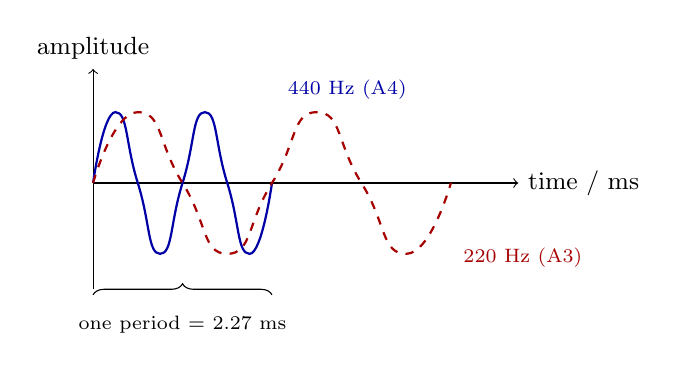
\begin{tikzpicture}[x=1cm,y=1cm]
  \draw[->] (0,0) -- (5.4,0) node[right] {\small time / ms};
  \draw[->] (0,-1.35) -- (0,1.45) node[above] {\small amplitude};
  \draw[thick,blue!65!black] plot[smooth,tension=1] coordinates {(0,0)(0.284,0.9)(0.568,0)(0.852,-0.9)(1.136,0)(1.42,0.9)(1.704,0)(1.988,-0.9)(2.272,0)};
  \draw[thick,red!65!black,dashed] plot[smooth,tension=1] coordinates {(0,0)(0.568,0.9)(1.136,0)(1.704,-0.9)(2.272,0)(2.84,0.9)(3.408,0)(3.976,-0.9)(4.544,0)};
  \node[blue!65!black,anchor=west] at (2.35,1.18) {\scriptsize 440 Hz (A4)};
  \node[red!65!black,anchor=west] at (4.58,-0.95) {\scriptsize 220 Hz (A3)};
  \draw[decorate,decoration={brace,amplitude=4pt},yshift=-2pt] (0,-1.35) -- (2.272,-1.35)
    node[midway,below=4pt] {\scriptsize one period = 2.27 ms};
\end{tikzpicture}

\small Figure 1-1. Halving the frequency doubles the period; 220 Hz and 440 Hz are one octave apart. The vertical axis is normalized amplitude, not sound-pressure level.
\end{center}

Pluck a 440 Hz string and a 220 Hz string together and you hear ``the same note, only higher and lower,'' not two unrelated sounds. The ear groups frequencies in a 2:1 ratio as the same pitch class, which is why note names repeat.

\section{Note names and the piano keyboard}

The seven white keys of a piano form one group, named C, D, E, F, G, A, B in order. Black keys sit between white keys and take a sharp (\sharpsym) or flat (\flatsym) name: C\sharpsym{} and D\flatsym{} are two names for the same key, an enharmonic pair.

\begin{center}
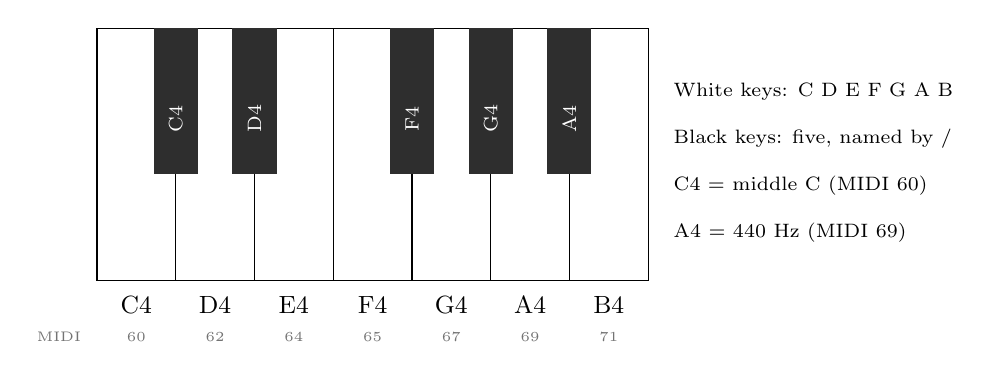
\begin{tikzpicture}[x=1cm,y=1cm,font=\small]
  \foreach \i/\n/\m in {0/C4/60,1/D4/62,2/E4/64,3/F4/65,4/G4/67,5/A4/69,6/B4/71} {
    \draw[fill=white] (\i,0) rectangle ++(1.0,3.2);
    \node at (\i+0.5,-0.32) {\n};
    \node[font=\tiny,text=black!55] at (\i+0.5,-0.72) {\m};
  }
  \node[anchor=east,font=\tiny,text=black!55] at (-0.08,-0.72) {MIDI};
  \foreach \x/\n in {0.72/C\sharpsym4,1.72/D\sharpsym4,3.72/F\sharpsym4,4.72/G\sharpsym4,5.72/A\sharpsym4} {
    \fill[black!82] (\x,1.35) rectangle ++(0.56,1.85);
    \node[white,font=\scriptsize,rotate=90] at (\x+0.28,2.05) {\n};
  }
  \node[anchor=west,font=\scriptsize] at (7.2,2.4) {White keys: C D E F G A B};
  \node[anchor=west,font=\scriptsize] at (7.2,1.8) {Black keys: five, named by \sharpsym/\flatsym};
  \node[anchor=west,font=\scriptsize] at (7.2,1.2) {C4 = middle C (MIDI 60)};
  \node[anchor=west,font=\scriptsize] at (7.2,0.6) {A4 = 440 Hz (MIDI 69)};
\end{tikzpicture}

\small Figure 1-2. Note names and MIDI numbers across one octave. Yeban's piano roll uses the same C4 = 60 convention as this keyboard.
\end{center}

The distance between two adjacent keys, including black keys, is a semitone. Two semitones make a whole tone. From C to the next C there are eight white keys and twelve semitones: one octave. On a piano there is no black key between E and F or between B and C, so those pairs are already a semitone apart; the other adjacent white keys are a whole tone apart.

\section{Scientific pitch notation and MIDI numbers}

The same note name recurs in every octave, so a number is required to make it unique. Scientific pitch notation names middle C as C4, then C5, C6 upward and C3, C2 downward. The number follows the letter and does not change with accidentals. Yeban and MIDI files both use C4 for middle C; this matches the pitch-range labels in the in-app manual.

MIDI encodes pitch as an integer from 0 to 127, with middle C = 60 and A4 = 69. The conversion is:

\begin{equation}
  n = 69 + 12\log_2\!\left(\frac{f}{440}\right),
  \qquad
  f = 440 \times 2^{(n-69)/12}.
  \label{eq:midi-frequency}
\end{equation}

Here \(n\) is the MIDI number and \(f\) is frequency in Hz. Equation \eqref{eq:midi-frequency} assumes 12-tone equal temperament and makes frequency and pitch number invertible. Substituting \(n=60\) gives about 261.63 Hz for C4; C5 is 523.25 Hz, exactly double.

\section{Twelve-tone equal temperament}

If an octave is exactly 2:1, dividing it into twelve equal semitones requires each semitone to multiply frequency by:

\begin{equation}
  r = 2^{1/12} \approx 1.059463.
  \label{eq:semitone-ratio}
\end{equation}

One semitone above A4 = 440 Hz is A\sharpsym4/B\flatsym4:

\[
  440 \times 2^{1/12} \approx 466.16\ \text{Hz}.
\]

This system is 12-tone equal temperament. It lets you transpose freely in any key with a uniform keyboard shape; the price is that, except for the octave, most intervals deviate slightly from the simple integer ratios of just intonation. Pop, rock, jazz, and Yeban's default pitch system all assume it.

\begin{table}[htbp]
\centering
\small
\caption{White-key frequencies in the octave of middle C (equal temperament, A4 = 440 Hz).}
\begin{tabular}{lccccccc}
\toprule
Note & C4 & D4 & E4 & F4 & G4 & A4 & B4 \\
\midrule
MIDI & 60 & 62 & 64 & 65 & 67 & 69 & 71 \\
Frequency/Hz & 261.63 & 293.66 & 329.63 & 349.23 & 392.00 & 440.00 & 493.88 \\
\bottomrule
\end{tabular}
\end{table}

\section{Note names, solfège, and numbered notation}

A pitch can be called by four common systems, each for a different job:

\begin{itemize}
  \item \textbf{Note names}: C, D, E, and so on are fixed names and do not change with key. Yeban's roll labels, MIDI files, and chord symbols use them.
  \item \textbf{Solfège}: do, re, mi, fa, sol, la, si. In fixed-do, C is always do; in movable-do, the tonic is do, so the pitch behind a syllable changes when the key changes.
  \item \textbf{Numbered notation}: 1–7 denote scale degrees, with 1 as the tonic. ``1 = C'' means C is the tonic. It is good for fast melodic shorthand but poor for exact chord inversions.
  \item \textbf{Scale degrees}: Roman I, II, III or Arabic numbers denote the position in a scale; this is the usual language of harmonic function.
\end{itemize}

Beginners most often confuse note names with solfège: note names are absolute, solfège is relative. Seeing C4 should first bring up ``middle C, MIDI 60, 261.63 Hz,'' not an automatic ``do''—C is sung as do only in C major with fixed-do.

\section{How to do it in Yeban}

\begin{enumerate}
  \item Press \texttt{P} or \texttt{F7} to open the piano roll; it is the first tab of the bottom console.
  \item The vertical axis is made of pitch rows. The default view shows 16 rows (C4–E\flatsym5), and only C anchors are labeled on the left; scroll up or down for higher or lower octaves. Row heights and note names come from the same pitch mapping, so there is no second coordinate system where a row looks like C4 but sounds like something else.
  \begin{center}
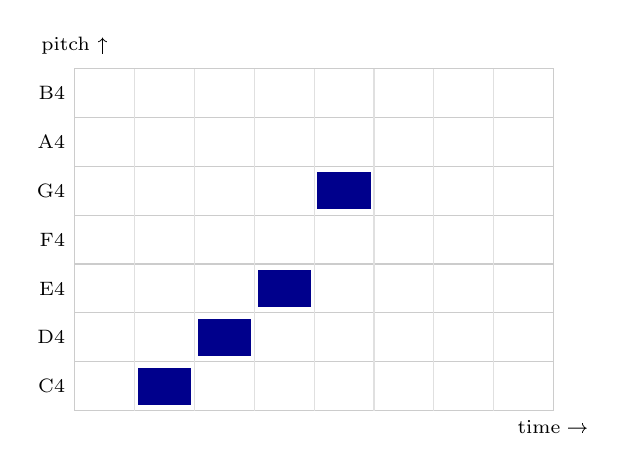
\begin{tikzpicture}[x=0.80cm,y=0.62cm]
  \foreach \r/\n in {0/C4,1/D4,2/E4,3/F4,4/G4,5/A4,6/B4} {
    \draw[black!20] (0,\r) rectangle (7.6,\r+1);
    \node[left,font=\scriptsize] at (0,\r+0.5) {\n};
  }
  \foreach \x in {0.95,1.9,2.85,3.8,4.75,5.7,6.65} {
    \draw[black!12] (\x,0) -- (\x,7);
  }
  \fill[blue!55!black] (1.0,0.12) rectangle (1.85,0.88);
  \fill[blue!55!black] (1.95,1.12) rectangle (2.80,1.88);
  \fill[blue!55!black] (2.90,2.12) rectangle (3.75,2.88);
  \fill[blue!55!black] (3.85,4.12) rectangle (4.70,4.88);
  \node[above,font=\scriptsize] at (0,7.1) {pitch ↑};
  \node[below,font=\scriptsize] at (7.6,0) {time →};
\end{tikzpicture}

\small Figure 1-3. Pitch rows in Yeban's piano roll. Time runs horizontally, pitch vertically; only C4--B4 are drawn here, while the default view shows 16 rows (C4--E\flatsym5).
\end{center}
\item Select a MIDI clip in the arrangement area, choose the draw tool (number key \texttt{2}), and click the C4 row to write a C4 note; drag to lengthen it.
  \item With a note selected, \texttt{↑}/\texttt{↓} transpose by a semitone and \texttt{Shift+↑}/\texttt{Shift+↓} by a whole octave. The note name and frequency follow Equation \eqref{eq:midi-frequency}.
  \item Press \texttt{Space} to play. Compare against an A4 = 440 Hz reference: your C4 should be nine semitones below it (60 versus 69).
\end{enumerate}



\screenshot{piano-roll-pitch-labels}{Piano-roll pitch labels against the piano keyboard}{Piano-roll pitch labels against the piano keyboard}

\textbf{Not yet available:} this volume does not describe spectrum analyzers or automatic pitch detection that Yeban does not currently provide. If a later version adds them, this section will link to them rather than show a button that does not exist.

\section{Pitch and register in real songs}

\begin{itemize}
  \item \textbf{Queen, ``Bohemian Rhapsody''}: The opening ballad sits in a warm mid-register piano-and-vocal zone before the operatic section leaps into falsetto highs and deep choral lows, using register span alone to create theatrical contrast.
  \item \textbf{Adele, ``Someone Like You''} (A major): The piano arpeggio holds the low-mid floor while the vocal stays intimate in the verse and climbs into the upper-mid range for the chorus, lifting emotion purely through pitch centre.
  \item \textbf{Jay Chou, ``Sunny Day'' (晴天)} (G major): Clean upper-fret acoustic guitar harmonics establish an immediate bright hook before the vocal enters in a close conversational mid-register.
\end{itemize}

\section{Exercises}


\begin{exercise}
\begin{enumerate}
  \item Give the note name for MIDI numbers 60, 64, 67, and 69.\\
  \emph{Answer:} C4, E4, G4, A4.
  \item Given A4 = 440 Hz, find the frequencies of A3 and C5.\\
  \emph{Hint:} A3 is one octave below A4, so halve the frequency; C5 is one octave above C4, which is about 261.63 Hz.\\
  \emph{Answer:} A3 = 220 Hz; C5 $\approx$ 523.25 Hz.
  \item How many semitones are there from C4 to G4?\\
  \emph{Answer:} Seven: C–C\sharpsym–D–D\sharpsym–E–F–F\sharpsym–G.
  \item Why is there no black key between E and F?\\
  \emph{Answer:} In the natural scale E–F is already a semitone; black keys only fill the semitones inside whole tones.
  \item In Yeban, write C4–D4–E4–G4–G4–F4–E4–D4, play with \texttt{Space}, then raise the last two notes by one semitone with \texttt{↑} and listen to the change.\\
  \emph{Hint:} Align to the C4 row first and click cell by cell with the draw tool; do not guess pitch by dragging.
\end{enumerate}
\end{exercise}

\section{Help topic map}

\begin{center}
\small
\setlength{\tabcolsep}{3pt}
\begin{longtable}{p{0.33\linewidth}p{0.44\linewidth}p{0.17\linewidth}}
\toprule
Section & In-app help anchor & Note \\
\midrule
\endhead
Four dimensions of sound & \texttt{music-theory-sound-dimensions} & concept \\
Note names and keyboard & \texttt{music-theory-note-names-keyboard} & Figure 1-2 \\
Octave and semitone & \texttt{music-theory-octave-semitone} & Figure 1-2 \\
Scientific pitch and MIDI & \texttt{music-theory-scientific-pitch-midi} & Equation \eqref{eq:midi-frequency} \\
Equal temperament & \texttt{music-theory-equal-temperament} & Table 1-1 \\
Note names, solfège, numbers & \texttt{music-theory-solfege-numbered-notation} & concept \\
How to do it in Yeban & \texttt{music-theory-piano-roll-pitch} & procedure \\
Exercises & \texttt{music-theory-ch1-practice} & answers above \\
\bottomrule
\end{longtable}
\end{center}

\section*{Further reading}
\begin{itemize}
  \item \textbf{Open Music Theory, “Pitches.”} \url{https://openmusictheory.github.io/pitches.html} — separates pitch, pitch class, frequency, and octave, adding the physical intuition behind this chapter.
  \item \textbf{YouTube, “The Harmonic Series \textbar{} The Language of Sound.”} \url{https://www.youtube.com/watch?v=NBB47aLlj88} — shows how overtones stack inside one note, connecting pitch with timbre.
\end{itemize}

